\documentclass[11pt, oneside]{article} 
\usepackage{geometry}
\geometry{letterpaper} 
\usepackage{graphicx}
	
\usepackage{amssymb}
\usepackage{amsmath}
\usepackage{parskip}
\usepackage{color}
\usepackage{hyperref}

\graphicspath{{/Users/telliott_admin/Tex/png/}}
% \begin{center} 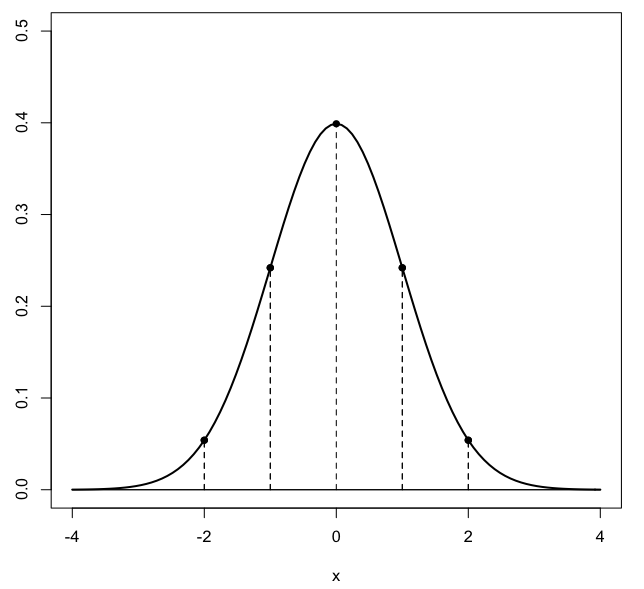
\includegraphics [scale=0.4] {gauss3.png} \end{center}

%break
\title{Bayes theorem}
\date{}

\begin{document}
\maketitle
\Large

The standard form of Bayes' Theorem (or law) is
\[ P(A|B) = \frac{P(B|A) \ P(A)}{P(B)} \]
where $P(A)$ is the probability of some event $A$ being true (and likewise for $P(B)$), and $P(A|B)$ is the conditional probability of $A$ being true, if it is already known, or \emph{given}, that $B$ is true.  (We read $P(A|B)$ as "the probability of $A$ given $B$").

\begin{center} 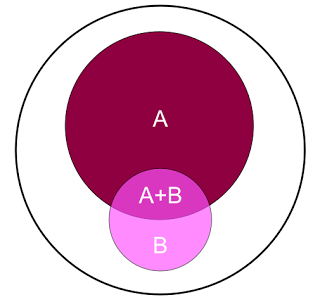
\includegraphics [scale=0.5] {bayes_circles.png} \end{center}

If we think of the black circle in the figure as encompassing our entire "event space", with a total area equal to 1, then the sizes of the colored regions represent probabilities.  In particular, the magenta region labeled A+B has area equal to the probability that both A and B are true.  This probability can be seen as equal to the area of A, $P(A)$, times the \emph{fraction of that area in which B is also true}.  This is the meaning of $P(B|A$).

The general equation form of Bayes' Theorem is symmetrical, and can be rearranged to give

\[ P(B) \ P(A|B) = P(A) \ P(B|A) = P(A,B) \]

where $P(A,B)$ is the probability that both $A$ and $B$ are true.

\subsection*{A slightly strained example}

As a more specific example, suppose that it is cloudy about half the time, and that when it is cloudy it rains about half the time.  Then
\[ P(rain,cloud) = P(rain|cloud) \ P(cloud) = 0.5 \times 0.5 = 0.25 \]

To better illustrate the utility of Bayes' Theorem, I need to make this example a little more complicated (and slightly unrealistic, but bear with me).  Have you ever felt the rain on a bright sunny day, looked up and thought, where the heck are the clouds?  We're going to say that it's nearly always cloudy when it's raining, but there are exceptional events.

Now, with this idea in mind and possessing just this data, we can't determine $P(rain)$, the unconditional probability of rain, since we don't know how often it rains when it's not (very) cloudy.  Let's say that rain when it's not cloudy is quite rare ($P = 0.01$), so then the total probability of rain is

\[ P(rain) = P(rain,cloud) + P(rain,not \ cloud) = 0.26 \]
Restating this
\[ P(rain) \ P(cloud|rain) = P(cloud) \ P(rain|cloud) \]
\[ 0.26 \times P(cloud|rain) = 0.5 \times 0.5 = 0.25 \]
\[ P(cloud|rain) = 0.25 / 0.26 \approx 0.96 \]

\subsection*{Sensitivity and Specificity}

In medical microbiology it's quite common to consider a test for some condition, e.g. an RADT for \emph{Streptococcus pyogenes} on a throat swab.  A typical value for the sensitivity of this test is $90\%$.  Sensitivity is about "classifying people with the disease correctly."  The stated value means that, with extensive knowledge (i.e. additional testing) of a similar population, it is known that $90\%$ of people with a Group A Strep pharyngitis will test positive.

Specificity is about "classifying people without the disease correctly."  For this particular test, the specificity is about $70\%$.  This means that $70\%$ of people (who complain of pharyngitis and thus are tested) but who do not have Group A Strep pharyngitis, will test negative.

These numbers sound pretty good, and in fact high percentages like these two values are commonly used as the basis for inferring that it is quite likely that someone with a positive test has a strep throat.  However, this inference is wrong.  Let's look at why that is the case.

In the figure below, the left panel is a key showing shapes and colors representing four types of people, those with or without the disease, and those with positive or negative test results.  As you can see, the stated values for sensitivity and specificity hold for this population, where each symbol represents an individual.

\begin{center} 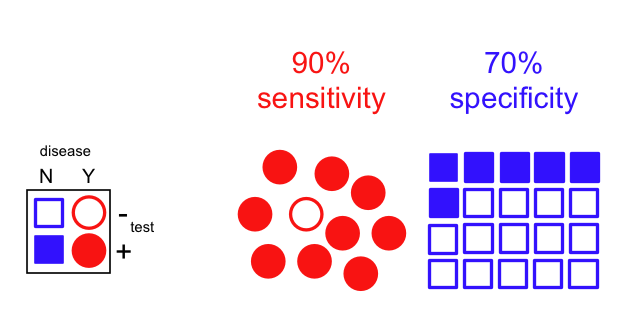
\includegraphics [scale=0.5] {radt.png} \end{center}

Now the question we (especially as patients) really want answered is this:  given that I have a positive test result, how likely is it that I have strep throat?  To find out, we first count up all the filled symbols, there are $9$ red ones and $6$ blue ones.  That's the total of positive tests.  What fraction of these are red?  The answer is $9/(6+9) = 60\%$.

That's pretty good, but we have (without being explicit about it) assumed an additional fact in coming to this conclusion.  That information is the \emph{prevalence}, the number of people with the disease in this population that has undergone testing.  Our assumption is that the prevalence is $1/3$;  there are twice as many blue symbols (both filled and unfilled) as red ones.  (One might quibble and call this the \emph{incidence}, if we think of this value as a rate per unit time).

However, the correct value for the prevalence in this scenario is actually $0.10$.  About $10\%$ of people who come into a doctor's office with acute pharyngitis and are tested actually have strep throat.  (The rest have a viral illness).

Here is that population

\begin{center} 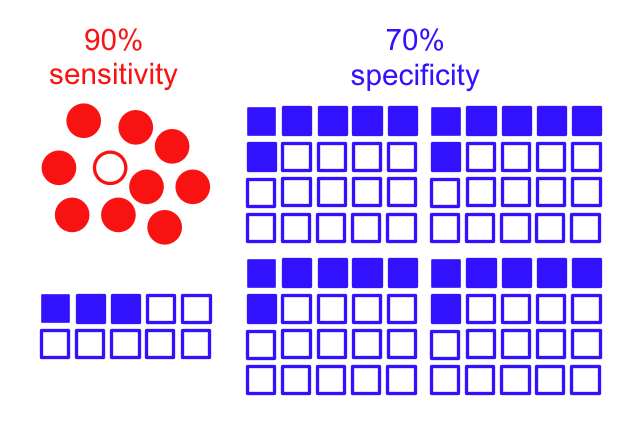
\includegraphics [scale=0.5] {radt2.png} \end{center}

Observe that the values for sensitivity and specificity are unchanged, but now the fraction of all symbols that are red symbols is only $10\%$.  As before, add up the total filled symbols and determine what fraction are red.  I obtain $9/(27 + 9) = 9/36 = 0.25$.  Restated:

\[ P(strep\ throat|positive\ test) \approx 0.25 \]

\subsection*{Leprechauns}

\begin{quote}\textcolor{blue}{I have a test machine that determines whether the subject is a flying leprechaun from Mars. I'm told the test is 99\% accurate. I put person after person into the machine and the result is always negative (correctly). Finally one day, I put someone (say, Tom Hanks) into the machine and the light comes on that says "Flying Leprechaun!" Would you believe the machine? Of course not: that would be ridiculous, so we conclude that we just happened to hit the 1\% where the test errs. We find it easy to completely reject a test result when it predicts something impossible (even if the test is very accurate); now we have to train ourselves to almost completely reject a test result when it predicts something almost completely impossible (even if the test is very accurate).}\end{quote}

This quote and many useful observations about statistics can be found at 

http://norvig.com/experiment-design.html

\begin{center} 
\includegraphics [scale=0.5] {norvig.png} \end{center}

\subsection*{More on sensitivity, etc.}

There are more mathematically sophisticated ways to obtain the results we obtained above, and these are especially useful when the numbers aren't so well-behaved.  One other way is to fill out a \emph{contingency table}.  Start by picking the total population size as a large enough number to make all the entries integers.  Here, $N=100$ is a good size.  The first step in construction of the table looks like this:

\[
\begin{matrix}
disease & healthy & total\\
 &  &  & pos\ test \\
 &  &  & neg\ test \\
\hline
 10 & 90  & 100 & total \\
\end{matrix}
\]

We have divided our $N=100$ into two groups, with and without disease, using the prevalence.  Next, incorporate the sensitivity

\[
\begin{matrix}
disease & healthy & total\\
 9  &  & & pos\ test \\
 1  &  & & neg\ test \\
\hline
 10 & 90  & 100 & total \\
\end{matrix}
\]

and the specificity

\[
\begin{matrix}
disease & healthy & total\\
 9  & 27 & & pos\ test \\
 1  & 63 & & neg\ test \\
\hline
 10 & 90  & 100 & total \\
\end{matrix}
\]

Last, sum along the rows to calculate the \emph{marginal} totals

\[
\begin{matrix}
disease & healthy & total\\
9 & 27 & 36 & pos\ test \\
1 & 63 & 64 & neg\ test \\
\hline
10 & 90 & 100 & total \\
\end{matrix}
\]

And as we said before, the predictive value of the test, the fraction of people with a positive test that actually have disease, is $9/36$.

\subsection*{Bayes' Theorem}

The third way to do the calculation is to use Bayes' Theorem directly.

\[ P(A|B) = \frac{P(B|A) \ P(A)}{P(B)} \]

In this example

\[ P(disease|pos\ test) = \frac{P(pos\ test|disease) \times P(disease)}{P(pos \ test)} \]
\[ P(disease|pos\ test) = \frac{sensitivity \times prevalence}{P(pos \ test)} \]

The denominator is the probability of a positive test under all models.
\[ P(pos \ test) = P(pos \ test|disease) \times P(disease) + P(pos \ test|healthy) \times P(healthy) \]
\[ = sensitivity \times prevalence + (1-specificity) \times (1-prevalence) \]

Plugging in the actual numbers I obtain:

\[ P(disease|pos\ test) = \frac{0.9 \times 0.1}{0.9 \times 0.1 + (1-0.70) \times (1-0.1)} \]
\[ = \frac{0.09}{0.09 + 0.27} = \frac{0.09}{0.36} = 0.25 \]

\subsection*{General form}
The RADT example shows the equation form of Bayes' Theorem and highlights how appropriate it seems for scientific reasoning.  The general form employs the terms \emph{model}  M or \emph{hypothesis} (H), and observed \emph{data} D.  We write
\[ P(H|D) = \frac{P(D|H) \times P(H)}{P(D)} \]

where $P(D)$ is the probability of the data under all models.  Here we have only two models, let's call them H1 (disease) and H2 (healthy).  Then we have
\[ P(H1|D) = \frac{P(D|H1) \times P(H1)}{P(D|H1) \times P(H1) + P(D|H2) \times P(H2) } \]


I will give an example below that I hope will make all this much clearer.  But for now, notice that $P(H1)$, the probability that the model (having disease) is correct, before we see any data or test results, is just the prevalence.  In technical lingo this is called the \emph{prior}.  Our prior or initial estimate of the probability of having disease is just the prevalence, or $10\%$.

This estimate will be updated after we see the results of the test.  The term $P(D|H1)$ is called the \emph{likelihood} or probability of seeing this data if model $H1$ is true.

The term on the bottom looks formidable (and it certainly is when the model parameters are continuous rather than discrete values, so that it becomes an integral), but it is really only there to make the probabilities come out to have a total equal to one.  That is, for real probabilities we need 

\[ P(H1) + P(H2) = 1 \]

and this awkward factor in the denominator is a normalizing constant to make the sum of all probabilities equal one.  We'll see how that actually works next.

\subsection*{The occasionally dishonest casino}

Consider an establishment that has nearly all honest, \emph{fair} dice (F) which, when rolled repeatedly, generate one through six at the expected frequency ($P = 1/6$  for each outcome).  However, rare dice are not fair but crooked or \emph{loaded} (L), and they generate six with a probability $P=1/2$, the other five outcomes occuring with equal probabilities $P=1/10$ for each one.

Now, suppose we know somehow that the frequency of loaded dice is $1/100$ (our prior knowledge).  We pick a die at random and generate some data.  We wish to calculate the probability that this die is loaded.  We roll three sixes in a row.  Wow!  How to calculate?

(This example comes from Durbin \emph{et al}., \emph{Biological Sequence Analysis}).

We write Bayes' formula:

\[ P(L|D) = \frac{P(D|L) \times P(L)}{P(D)} \]
\[ = \frac{P(D|L) \times P(L)}{P(D|L) \times P(L) + P(D|F) \times P(F)} \]

We have:

\[ P(D|L) = (0.5)^3 = 0.125 \]
\[ P(L) = 0.01 \]
\[ P(D|L) \times P(L) = 0.00125 \]
\[ P(D|F) = (1/6)^3 \approx 0.0046296 \]
\[ P(F) = 0.99 \]
\[ P(D|F) \times P(F) \approx 0.004583 \]

Plugging in:

\[ P(L|D) = \frac{P(D|L) \times P(L)}{P(D)} \]
\[ = \frac{P(D|L) \times P(L)}{P(D|L) \times P(L) + P(D|F) \times P(F)} \]
\[ P(L|D) = \frac{0.00125}{0.00125 + 0.004583} \approx 0.214 \]

In Bayesian terminology we would say that our prior for the hypothesis that this die is loaded was $0.01$, but now after seeing three sixes in a row, we have updated to a posterior probability that the die is loaded equal to $0.21$.  However, it is still much more likely than not that the die is a fair one (because the loaded type was so rare to begin with).  

Suppose we roll again.  \emph{Another} six.  Now we update our prior (the 0.01 from before becomes 0.214).  We have

\[ P(D|L) = 0.5 \]
\[ P(L) = 0.214 \]
\[ P(D|F) = 0.166 \]
\[ P(F) = 0.99 \]

Plugging in:

\[ P(L|D) = \frac{P(D|L) \times P(L)}{P(D)}  \]
\[ = \frac{P(D|L) \times P(L)}{P(D|L) \times P(L) + P(F|L) \times P(F)} \]
\[ P(L|D) = \frac{0.5 \times 0.214}{0.5 \times 0.214 + 0.166 \times 0.99} \approx 0.39 \]

It is only after obtaining one more six, for a total of five sixes in a row, that that it becomes more likely than not that the die is loaded.  

This business of updating the prior at each round makes the calculation somewhat tedious.  There is an easier way which uses the \emph{odds form} of Bayes' formula.

\[ O(L) = \frac{P(L)}{P(F)} \]
\[ O(L|D) = O(L) \times Likelihood\  ratio  \]

where the likelihood of F is $P(D|F)$ and the likelihood of L is $P(D|L)$.  For each successive six that is rolled, we have the same ratio

\[ ratio = \frac{P(D|L)}{P(D|F)} = \frac{1/2}{1/6} =  3 \]

With 3 sixes in a row, that factor is $3 \times 3 \times 3 = 27$, and the odds of the die being loaded are $1/99 \times 27 = 27/99$.  To convert the odds to probability

\[ O(L) = \frac{P(L)}{P(F)} = \frac{P(L)}{1-P(L)} \]

Odds are usually expressed as $n:d$ but we can write them as $n/d$

\[ \frac{n}{d} = \frac{P(L)}{1-P(L)} \]
\[ \frac{n}{d} \times (1-P(L)) = P(L) \]
\[  \frac{n}{d} =  \frac{n+d}{d} \times P(L) \]
\[ P(L) = \frac{n}{n+d} \]
\[ P(L) = 27/126 \approx 0.214 \]

This matches what we had from Bayes' Rule above.  For 4 sixes in a row we have a factor of 81 and
\[ P(L) = 81/(99 + 81) = 0.45 \]
For 5 sixes in a row we have a factor of 243 and calculate
\[ P(L) = 243/(99 + 243) = 0.71 \]

Perhaps you've been thinking that this example doesn't have much to do with biology.  Think of the crooked die as a particular 12 bp segment of DNA that might be a transcription factor binding site.  You wish to estimate the probability that a particular sequence really is such a site.  Do you have an idea about how to proceed?

\subsection*{Variable-sided dice}

I have one more example before we quit (it's from Allen Downey's book \emph{Think Bayes}), and it helps to illustrate more clearly some of the things we've already touched on.  The example is a set of dice (five in all) that are either 4-sided (with numbers 1 to 4), 6-sided, 8-sided, 12-sided or 20-sided.  I have a bag containing one die of each type.  I reach in and randomly draw one of the dice, and without showing you which one it is, roll a six (it's my lucky day).  What are the probabilities?

\[ P(six|4) = 0  \]
\[ P(six|6) = \frac{1}{6}  \]
\[ P(six|8) = \frac{1}{8}  \]
\[ P(six|12) = \frac{1}{12}  \]
\[ P(six|20) = \frac{1}{20}  \]

Now, the prior for each was $1/5$.  But $P(six|4) = 0$ so clearly there is no chance that this die is the 4-sided die.  Now we calculate

\[ P(six|6) \times P(6) = \frac{1}{6} \times \frac{1}{5} = 1/30 \]
\[ P(six|8) \times P(8) = \frac{1}{8} \times \frac{1}{5} = 1/40 \]
\[ P(six|12) \times P(12) = \frac{1}{12} \times \frac{1}{5} = 1/60 \]
\[ P(six|20) \times P(20) = \frac{1}{20} \times \frac{1}{5} = 1/100 \]

These probabilities have the correct proportions.  The probability that the die was the 6-sided one is twice the probability that it was the 12-sided one.  However, to make these true probabilities, we must normalize so that if the probability for every possible event is added up, so that we obtain $P=1.0$ for all the possibilities together.  The way to do that is to divide each probability above by the sum of all of them.

The sum is 
\[ \frac{1}{30} + \frac{1}{40} + \frac{1}{60} + \frac{1}{100} =  0.085  \]

For example, the probability that we picked the 6-sided die, given that we obtained a six on the roll, is
\[ P(6|six) = \frac{1/30}{0.085} \approx  0.39 \]

So I hope that with this example, you can see finally what this is about

\[ P(H1|D) = \frac{P(D|H1) \times P(H1)}{P(D|H1) \times P(H1) + P(D|H2) \times P(H2) + P(D|H3) \times P(H3) } \]
\[ P(H1|D) = \frac{P(D|H1) \times P(H1)}{\Sigma_i P(D|H_i) \times P(H_i) } \]

That scary term in the denominator is just a way of making our probabilities sum to $1$.  And the beauty of modern approaches to Bayes is that, using techniques like Markov Chain Monte Carlo (MCMC) we can avoid calculating that denominator altogether.  That ability leads to very useful techniques and results.

Finally, it is worth pointing out how important it is that one obtain (if possible) data that contradicts a hypothesis completely, as in the situation with the 4-sided dice and an observation of six.  However, it is also possible to proceed on the basis of the probability that a hypothesis is correct.  To me, this seems eminently sensible, but it would be anathema to Sir Ronald Fisher.  In conclusion consider this xkcd cartoon:

\begin{center} 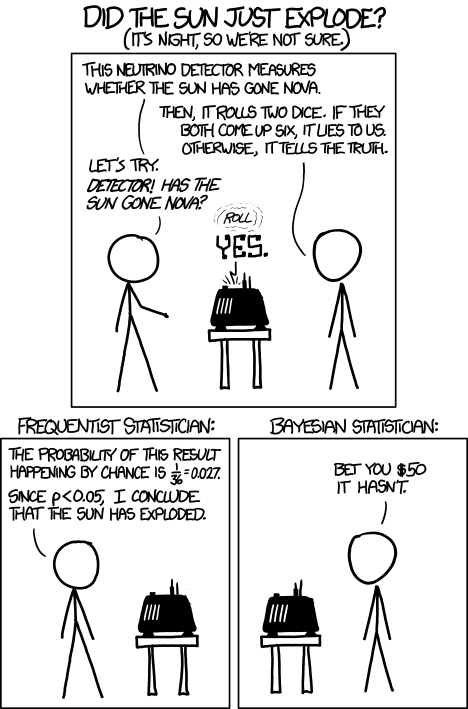
\includegraphics [scale=0.4] {frequentists_vs_bayesians.png} \end{center}


\end{document}  